\chapter{\modelname{}: Our Approach}
\label{ch:emotx}

\begin{figure*}[t]
\centering
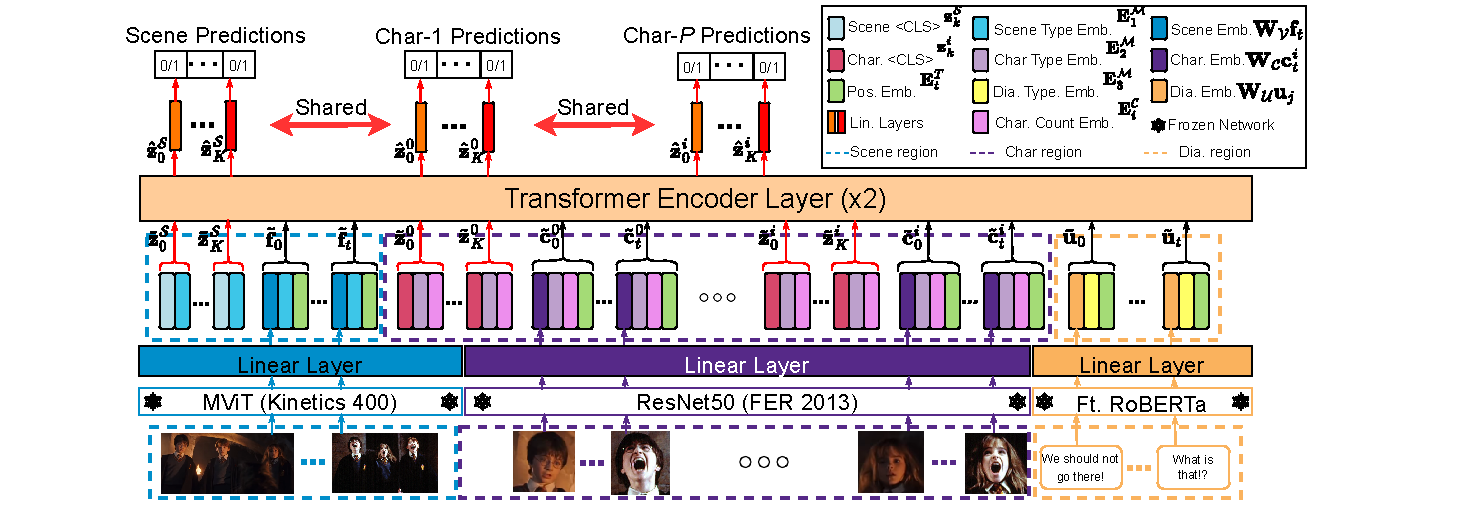
\includegraphics[width=\textwidth,height=0.33\textheight]{Figures/emotx_marked.pdf}
\vspace{-6mm}
\caption{An overview of \modelname{}.
\textbf{A}: Video features (in blue region),
character face features (in purple region), and
utterance features (in orange region)
are obtained using frozen backbones and projected with linear layers into a joint embedding space.
\textbf{B}: Here appropriate embeddings are added to the tokens to distinguish between modalities, character count, and to provide a sense of time.
We also create per-emotion classifier tokens associated with the scene or a specific character.
\textbf{C}: Two Transformer encoder layers perform self-attention across the sequence of input tokens.
\textbf{D}: Finally, we tap the classifier tokens to produce output probability scores for each emotion through a linear classifier shared across the scene and characters.}
\label{fig:model_overview}
\vspace{-3mm}
\end{figure*}

In this chapter, we introduce \modelname{}, a sophisticated method designed to jointly predict multi-label emotions and mental states for both movie scenes and individual characters within the scene. \modelname{} utilizes a Transformer-based architecture to achieve accurate and comprehensive emotion recognition.

The process begins with video pre-processing and feature extraction pipeline. This initial phase is crucial for distilling relevant representations from the complex visual and auditory information embedded in movie scenes. By carefully extracting key features, \modelname{} sets the stage for a more nuanced understanding of the emotional dynamics at play.

The core of \modelname{} lies in its Transformer encoder, that facilitates the seamless integration of information across various modalities. This encoder enables the model to capture intricate relationships and dependencies within the feature representations essential to capture the emotions. The Transformer architecture is particularly adept at handling sequential and contextual information, making it well-suited for the complex nature of emotional expression in movie scenes.

Building on these integrated representations, \modelname{} incorporates a classification module, drawing inspiration from prior advancements in multi-label classification with Transformers~\cite{q2l}. This module serves as the final computational layer, responsible for making predictions about emotions associated with each scene and character. By leveraging the Transformer's capacity for contextual understanding, \modelname{} excels in discerning the intricate nuances of emotions, providing a robust framework for comprehensive emotion recognition in the realm of cinematic storytelling.

An overview of the approach is presented in Fig.~\ref{fig:model_overview}.
